\documentclass[]{article}
\usepackage{lmodern}
\usepackage{amssymb,amsmath}
\usepackage{ifxetex,ifluatex}
\usepackage{fixltx2e} % provides \textsubscript
\ifnum 0\ifxetex 1\fi\ifluatex 1\fi=0 % if pdftex
  \usepackage[T1]{fontenc}
  \usepackage[utf8]{inputenc}
\else % if luatex or xelatex
  \ifxetex
    \usepackage{mathspec}
  \else
    \usepackage{fontspec}
  \fi
  \defaultfontfeatures{Ligatures=TeX,Scale=MatchLowercase}
\fi
% use upquote if available, for straight quotes in verbatim environments
\IfFileExists{upquote.sty}{\usepackage{upquote}}{}
% use microtype if available
\IfFileExists{microtype.sty}{%
\usepackage[]{microtype}
\UseMicrotypeSet[protrusion]{basicmath} % disable protrusion for tt fonts
}{}
\PassOptionsToPackage{hyphens}{url} % url is loaded by hyperref
\usepackage[unicode=true]{hyperref}
\hypersetup{
            pdfborder={0 0 0},
            breaklinks=true}
\urlstyle{same}  % don't use monospace font for urls
\usepackage{color}
\usepackage{fancyvrb}
\newcommand{\VerbBar}{|}
\newcommand{\VERB}{\Verb[commandchars=\\\{\}]}
\DefineVerbatimEnvironment{Highlighting}{Verbatim}{commandchars=\\\{\}}
% Add ',fontsize=\small' for more characters per line
\newenvironment{Shaded}{}{}
\newcommand{\KeywordTok}[1]{\textcolor[rgb]{0.00,0.44,0.13}{\textbf{#1}}}
\newcommand{\DataTypeTok}[1]{\textcolor[rgb]{0.56,0.13,0.00}{#1}}
\newcommand{\DecValTok}[1]{\textcolor[rgb]{0.25,0.63,0.44}{#1}}
\newcommand{\BaseNTok}[1]{\textcolor[rgb]{0.25,0.63,0.44}{#1}}
\newcommand{\FloatTok}[1]{\textcolor[rgb]{0.25,0.63,0.44}{#1}}
\newcommand{\ConstantTok}[1]{\textcolor[rgb]{0.53,0.00,0.00}{#1}}
\newcommand{\CharTok}[1]{\textcolor[rgb]{0.25,0.44,0.63}{#1}}
\newcommand{\SpecialCharTok}[1]{\textcolor[rgb]{0.25,0.44,0.63}{#1}}
\newcommand{\StringTok}[1]{\textcolor[rgb]{0.25,0.44,0.63}{#1}}
\newcommand{\VerbatimStringTok}[1]{\textcolor[rgb]{0.25,0.44,0.63}{#1}}
\newcommand{\SpecialStringTok}[1]{\textcolor[rgb]{0.73,0.40,0.53}{#1}}
\newcommand{\ImportTok}[1]{#1}
\newcommand{\CommentTok}[1]{\textcolor[rgb]{0.38,0.63,0.69}{\textit{#1}}}
\newcommand{\DocumentationTok}[1]{\textcolor[rgb]{0.73,0.13,0.13}{\textit{#1}}}
\newcommand{\AnnotationTok}[1]{\textcolor[rgb]{0.38,0.63,0.69}{\textbf{\textit{#1}}}}
\newcommand{\CommentVarTok}[1]{\textcolor[rgb]{0.38,0.63,0.69}{\textbf{\textit{#1}}}}
\newcommand{\OtherTok}[1]{\textcolor[rgb]{0.00,0.44,0.13}{#1}}
\newcommand{\FunctionTok}[1]{\textcolor[rgb]{0.02,0.16,0.49}{#1}}
\newcommand{\VariableTok}[1]{\textcolor[rgb]{0.10,0.09,0.49}{#1}}
\newcommand{\ControlFlowTok}[1]{\textcolor[rgb]{0.00,0.44,0.13}{\textbf{#1}}}
\newcommand{\OperatorTok}[1]{\textcolor[rgb]{0.40,0.40,0.40}{#1}}
\newcommand{\BuiltInTok}[1]{#1}
\newcommand{\ExtensionTok}[1]{#1}
\newcommand{\PreprocessorTok}[1]{\textcolor[rgb]{0.74,0.48,0.00}{#1}}
\newcommand{\AttributeTok}[1]{\textcolor[rgb]{0.49,0.56,0.16}{#1}}
\newcommand{\RegionMarkerTok}[1]{#1}
\newcommand{\InformationTok}[1]{\textcolor[rgb]{0.38,0.63,0.69}{\textbf{\textit{#1}}}}
\newcommand{\WarningTok}[1]{\textcolor[rgb]{0.38,0.63,0.69}{\textbf{\textit{#1}}}}
\newcommand{\AlertTok}[1]{\textcolor[rgb]{1.00,0.00,0.00}{\textbf{#1}}}
\newcommand{\ErrorTok}[1]{\textcolor[rgb]{1.00,0.00,0.00}{\textbf{#1}}}
\newcommand{\NormalTok}[1]{#1}
\usepackage{graphicx,grffile}
\makeatletter
\def\maxwidth{\ifdim\Gin@nat@width>\linewidth\linewidth\else\Gin@nat@width\fi}
\def\maxheight{\ifdim\Gin@nat@height>\textheight\textheight\else\Gin@nat@height\fi}
\makeatother
% Scale images if necessary, so that they will not overflow the page
% margins by default, and it is still possible to overwrite the defaults
% using explicit options in \includegraphics[width, height, ...]{}
\setkeys{Gin}{width=\maxwidth,height=\maxheight,keepaspectratio}
\IfFileExists{parskip.sty}{%
\usepackage{parskip}
}{% else
\setlength{\parindent}{0pt}
\setlength{\parskip}{6pt plus 2pt minus 1pt}
}
\setlength{\emergencystretch}{3em}  % prevent overfull lines
\providecommand{\tightlist}{%
  \setlength{\itemsep}{0pt}\setlength{\parskip}{0pt}}
\setcounter{secnumdepth}{0}
% Redefines (sub)paragraphs to behave more like sections
\ifx\paragraph\undefined\else
\let\oldparagraph\paragraph
\renewcommand{\paragraph}[1]{\oldparagraph{#1}\mbox{}}
\fi
\ifx\subparagraph\undefined\else
\let\oldsubparagraph\subparagraph
\renewcommand{\subparagraph}[1]{\oldsubparagraph{#1}\mbox{}}
\fi

% set default figure placement to htbp
\makeatletter
\def\fps@figure{htbp}
\makeatother


\date{}

\begin{document}

SiScLab 2018 Student Project \textbf{Analysis Tool for Materials
Design}. Written in Python3.

Authors: \href{https://github.com/Irratzo}{Johannes Wasmer},
\href{https://github.com/ChristianPartmann}{Christian Partmann}, and
\href{https://github.com/PraneethKatta}{Praneeth Katta}.

\section{Overview}\label{overview}

This subfolder \texttt{studentproject18ws} is currently a largely
independent side-project accompanying the main module
\texttt{masci-tools}. It was created in a student project, and consists
of three submodules:

\begin{itemize}
\tightlist
\item
  preprocessor: a HDF reader interface, and one implementation for
  \href{http://www.judft.de}{Fleur} band structure simulation output
\item
  visualization: a plotting interface, and one implementation for
  \href{http://www.judft.de}{Fleur} bandstructure+DOS plots
\item
  frontends: a Desktop GUI and a Web Dashboard (Tk and Jupyter) for
  interactive Fleur bandDOS plots.
\end{itemize}

A more thorough description and example use cases can be found in the
project \href{./doc/report.pdf}{report} and
\href{./doc/presentation.pdf}{presentation}.

\begin{figure}
\centering
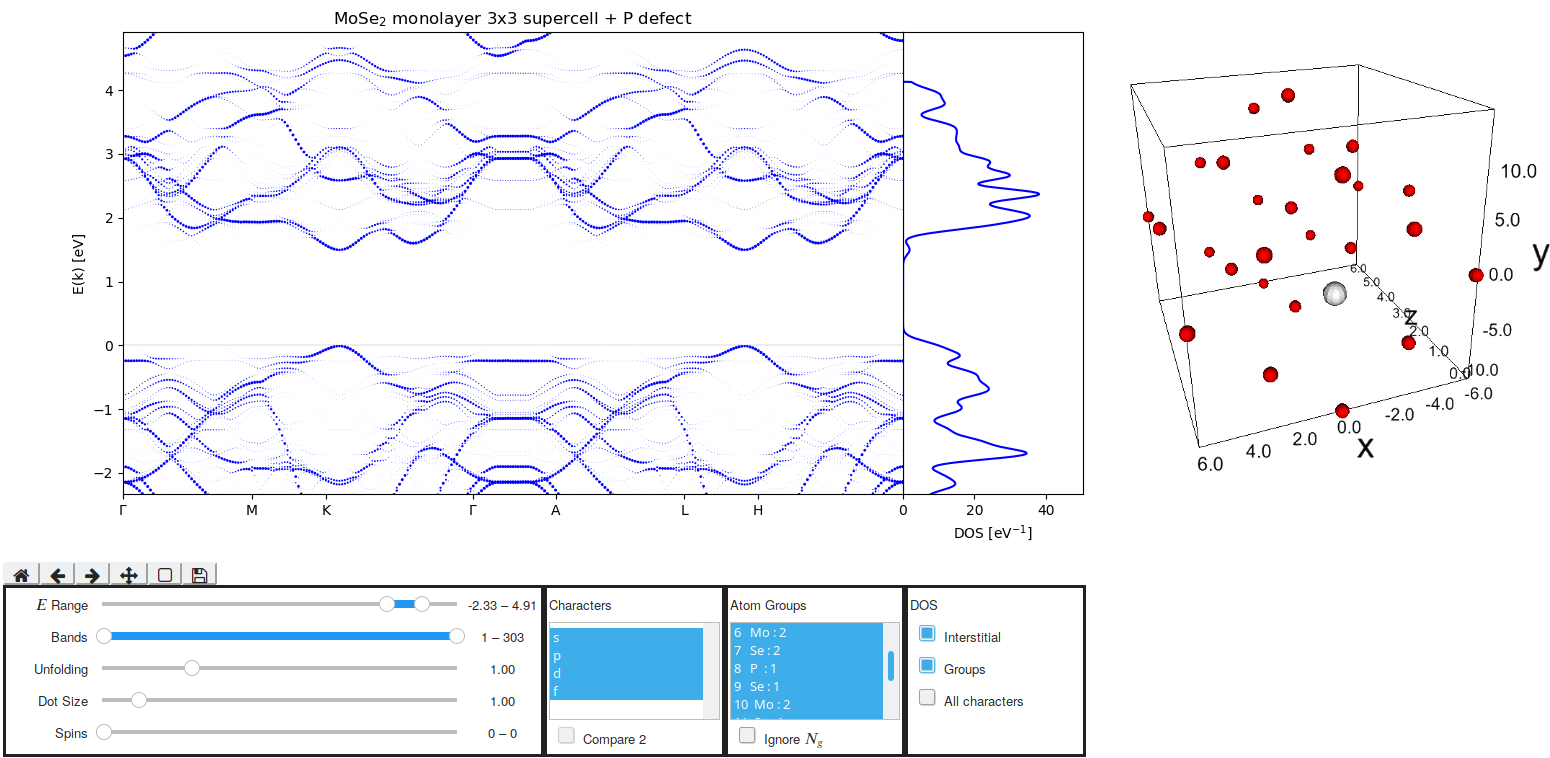
\includegraphics{./readme/web_frontend.png}
\caption{}
\end{figure}

\section{For Frontend Users}\label{for-frontend-users}

\subsection{General Remarks}\label{general-remarks}

These remarks apply to all frontends.

Though the Desktop and Web Frontend are functionally identical, there
might be small differences in how the controls are used and how they are
labeled.

\subsubsection{File Input}\label{file-input}

The frontends currently expects band structure data in the HDF output
format of \href{http://www.judft.de}{Fleur}. The density of states data
is expected to be in the CSV output format of
\href{http://www.judft.de}{Fleur}, one file per spin. If no density of
states files are supplied, the frontend will just draw a band structure
plot (BandPlot) and omit the adjoined density of states plot (DOSPlot).
Thus, in the following BandDOSPlot stands for both kinds of plot. The
Web Frontend will only show controls for data that is present in the
input (e.g., DOS and spin controls).

\subsection{Desktop Frontend}\label{desktop-frontend}

\subsubsection{Installation}\label{installation}

A windows executable file (.exe) is made by packing all the required
packages into the file. Any modern PC running on windows can run the
frontend without any installation process and there is no prerequisite
to execute this executable file. PC need not have python or other
packages installed.

For executables for other operating systems, please contact the
developers.

\subsubsection{Usage}\label{usage}

Desktop based front end GUI is easy to use. By just running the .exe
file provided will open the software with the packages involved to run
the software. There are three tabs/windows in the software. In the first
tab, absolute paths to the input data files must be entered in this
order: HDF and (optional) DOS file for spin 0 and 1.

Controls for all plots:

\begin{itemize}
\tightlist
\item
  Atom Groups: draw the BandDOSPlot only for the selected symmetry
  groups.
\item
  Character: select one or more band Characters (orbitals)
  `S',`P',`D',`F'.
\item
  Spin: select any one spin or both spins.
\item
  Marker size: Default marker size of 1.0 is selected. How ever, user
  have a choice to increase the marker size of the dots (eigenenergies)
  plotted in the BandPlot.
\item
  Ymin, Ymax: This control is used to limit the range energy range of
  the BandDOSPlot.
\item
  BandMin, BandMax: This control is used to limit the band range of the
  BandDOSPlot.
\item
  Update, SaveButton: Update the BandDOSplot to the newly selected data
  by user. Save the the plot as a PDF on disk.
\item
  Exponential weight: The unfolding exponent for supercell calculations
  (see \href{./doc/report.pdf}{report}). Value 0.0 means no unfolding.
  If the calculation is done with a unit cell, this control has no
  effect.
\item
  Compare 2Characters: When a user wants to compare 2 characters, this
  button makes the BandPlot show the influence of each character to each
  eigenergy using a sequential (2** colormap. The control is disabled if
  other than two characters are selected.
\item
  Ignore Atom group: This button allows an option to ignore the atom
  groups.
\end{itemize}

Controls for the DOSPlot only:

\begin{itemize}
\tightlist
\item
  Select groups: include selected atom groups in the DOS
\item
  Interstitial: include the interstitial in the DOS
\item
  All characters: include all characters in the DOS regardless of
  character selection. In the DOS CSV file, different input data is used
  (a summed column).
\end{itemize}

After the Update button is clicked, a BandPlot or BandDOS plot is
produced in Tab 2. A 3D atomic plot is produced in Tab 3.

\subsubsection{Troubleshooting}\label{troubleshooting}

If the BandPlot is not visible:

\begin{itemize}
\tightlist
\item
  Check if the three input files (if any) are belonging to the same
  Fleur calculation and selected appropriately.
\item
  Check if at least one Atom Group, one Character, one Spin is selected.
\item
  Check if Ymin is less than Ymax and similarly BandMin is less than
  BandMax such that software is able to plot.
\end{itemize}

Click on Update once again. If problem persists, restarting of the
software would be last attempt for making it work. Please open an issue
or contact the developers if the problem persists.

\subsection{Web Frontend}\label{web-frontend}

\subsubsection{Access}\label{access}

The Web Frontend is a Jupyter Dashboard. It is in experimental state (no
fileupload yet). You can try it out
\href{https://mybinder.org/v2/gh/JuDFTteam/masci-tools/studentproject18ws?filepath=studentproject18w\%2Ffrontend\%2Fjupyter\%2Fdemo\%2Fbinder_demo.ipynb}{here
on Binder}. You can run it locally (see developer section). If you have
an {[}AiiDaLab
account{]}(https://aiidalab.materialscloud.org/hub/login**: the
dashboard is planned to be published as an app there.

\subsubsection{Usage}\label{usage-1}

Using the Dashboard should be self-explanatory to the domain user. Some
tips:

\begin{itemize}
\tightlist
\item
  unlike the Desktop frontend, plot updates are instantaneous.
\item
  multi-selection boxes: use ctrl or shift to select multiple items.
\item
  slider values can also be typed into the adjoining text box.
\item
  should the app ever appear to get stuck, a reload/rerun will do the
  trick.
\item
  unlike the Desktop Frontend, empty selections are impossible.
\end{itemize}

\section{For Developers}\label{for-developers}

\subsection{Installation}\label{installation-1}

Though \texttt{masci-tools} is availabe via PyPI, there is currently no
plan to integrate \texttt{studentproject18ws}. If you want to use it in
your code, clone the repo, use it in an IDE, or append the path to your
\texttt{sys.path}:

\begin{Shaded}
\begin{Highlighting}[]
\ImportTok{import}\NormalTok{ sys}
\ControlFlowTok{if}\NormalTok{ path_repo }\KeywordTok{not} \KeywordTok{in}\NormalTok{ sys.path:}
\NormalTok{    sys.path.append(path_repo)}
    
\CommentTok{# now import works}
\ImportTok{from}\NormalTok{ studentproject18w.hdf.reader }\ImportTok{import}\NormalTok{ Reader}
\CommentTok{# ...}
\end{Highlighting}
\end{Shaded}

\subsubsection{Create project virtual
environment}\label{create-project-virtual-environment}

With conda (recommended): -
\href{https://www.anaconda.com/download}{Install Anaconda (3
recommended)} - Install the environment \texttt{masci-stupro} with the
necessary and recommended dependencies:

\begin{Shaded}
\begin{Highlighting}[]
\ExtensionTok{conda}\NormalTok{ create -f environment.yml}
\BuiltInTok{source}\NormalTok{ activate masci-stupro}
\end{Highlighting}
\end{Shaded}

With virtualenv (untested):

\begin{Shaded}
\begin{Highlighting}[]
\ExtensionTok{virtualenv}\NormalTok{ masci-stupro}
\BuiltInTok{source}\NormalTok{ masci-stupro/bin/activate}
\ExtensionTok{pip}\NormalTok{ install -r requirements_pip.txt }\CommentTok{# install requirements}
\end{Highlighting}
\end{Shaded}

\subsection{Programmatic use}\label{programmatic-use}

In this example, a Fleur HDF file is preprocessed using the Recipe
\texttt{FleurBands}. The resulting output \texttt{data} with the
extracted and transformed HDF datasets and attached load methods
(Extract-Transform-Load) is then passed to a plotter, alongside some DOS
CSV files for a bandstructure plot using \texttt{matplotlib} as backend
library.

\begin{Shaded}
\begin{Highlighting}[]
\ImportTok{import}\NormalTok{ matplotlib.pyplot }\ImportTok{as}\NormalTok{ plt}
\ImportTok{from}\NormalTok{ studentproject18w.hdf.reader }\ImportTok{import}\NormalTok{ Reader}
\ImportTok{from}\NormalTok{ studentproject18w.hdf.recipes }\ImportTok{import}\NormalTok{ Recipes}
\ImportTok{from}\NormalTok{ studentproject18w.plot.matplot }\ImportTok{import}\NormalTok{ BandDOSPlot}

\NormalTok{data }\OperatorTok{=} \VariableTok{None}
\NormalTok{reader }\OperatorTok{=}\NormalTok{ Reader(filepath}\OperatorTok{=}\NormalTok{filepath_hdf)}
\ControlFlowTok{with}\NormalTok{ reader }\ImportTok{as}\NormalTok{ h5file:}
\NormalTok{    data }\OperatorTok{=}\NormalTok{ reader.read(recipe}\OperatorTok{=}\NormalTok{Recipes.FleurBands)}
    \CommentTok{#}
    \CommentTok{# Note:}
    \CommentTok{# Inside the with statement (context manager),}
    \CommentTok{# all data attributes that are type h5py Dataset are available (in-file access)}
    \CommentTok{# When the statement is left,the HDF5 file gets closed and the datasets are closed.}
    \CommentTok{#}
    \CommentTok{# Use data outside the with-statement (in-memory access: all HDF5 datasets converted to numpy ndarrays):}
\NormalTok{    data.move_datasets_to_memory()}

\NormalTok{plotter }\OperatorTok{=}\NormalTok{ BandDOSPlot(plt, data, filepaths_dos)}
\NormalTok{(fig, ax_bands, ax_dos) }\OperatorTok{=}\NormalTok{ plter.setup_figure(fig_ratio}\OperatorTok{=}\NormalTok{[}\DecValTok{12}\NormalTok{,}\DecValTok{6}\NormalTok{], fig_scale}\OperatorTok{=}\DecValTok{1}\NormalTok{, fig_title}\OperatorTok{=}\StringTok{"BandDOS"}\NormalTok{)}
\NormalTok{data_selection }\OperatorTok{=}\NormalTok{ some_selection_process()}
\NormalTok{plotter.plot_bandDOS(}\OperatorTok{*}\NormalTok{data_selection)}
\NormalTok{plt.show()}
\end{Highlighting}
\end{Shaded}

\subsection{Try out Web Frontend
locally}\label{try-out-web-frontend-locally}

The demo notebook with the Dashboard is
\texttt{studentproject18w/frontend/jupyter/demo/demo.ipynb}.

\subsubsection{If using Jupyter
Notebook}\label{if-using-jupyter-notebook}

If using Windows, omit keyword \texttt{source}.

\begin{Shaded}
\begin{Highlighting}[]
\BuiltInTok{source}\NormalTok{ activate masci-stupro}
\BuiltInTok{cd}\NormalTok{ mypath/masci-tools/studentproject18ws/}
\ExtensionTok{jupyter-notebook}\NormalTok{ .}
\CommentTok{# if Home is not set to this dir, try this instead:}
\CommentTok{# /home/you/anaconda3/envs/myenv/bin/python /home/you/anaconda3/envs/myenv/bin/jupyter-notebook .}
\end{Highlighting}
\end{Shaded}

\subsubsection{If using Jupyter Lab}\label{if-using-jupyter-lab}

Additional installation step needed:

\begin{Shaded}
\begin{Highlighting}[]
\BuiltInTok{source}\NormalTok{ activate masci-stupro}
\ExtensionTok{jupyter}\NormalTok{ labextension install @jupyter-widgets/jupyterlab-manager jupyter-matplotlib ipyvolume}
\BuiltInTok{cd}\NormalTok{ mypath/masci-tools/studentproject18ws/}
\ExtensionTok{jupyter-lab}
\end{Highlighting}
\end{Shaded}

\subsection{Frontend Deployment}\label{frontend-deployment}

\subsubsection{Desktop Frontend}\label{desktop-frontend-1}

To create executables for different operating systems, use
\href{https://www.pyinstaller.org/}{PyInstaller}. The target file is
\texttt{frontend/tkinter/gui.py}.

\subsubsection{Web Frontend}\label{web-frontend-1}

The Web Frontend is currently a single Jupyter Notebook. In order to
publish it as a usable standalone app, additional work has to be done.

\begin{itemize}
\tightlist
\item
  (recommended: create \texttt{frontend/jupyter/Dashboard.py} widget and
  put code of
  \href{./frontend/jupyter/demo/demo_backend.ipynb}{demo\_back.ipynb}
  notebook inside it. Use
  \href{https://github.com/aiidalab/aiidalab-widgets-base/blob/master/aiidalab_widgets_base/structures.py}{aiidalab-widgets-base
  \textgreater{} StructureUploadWidget} as a template. Create
  \texttt{frontend/jupyter/Dashboard.ipynb} notebook. Use
  \href{https://github.com/aiidalab/aiidalab-widgets-base/blob/master/structures.ipynb}{StructureUploadWidget
  Demo Notebook} as a template.)
\item
  Add \href{https://pypi.org/project/fileupload/}{fileupload} to widget
  (again, like in StructureUploadWidget. See
  \href{./frontend/jupyter/demo/binder_fileupload_test.ipynb}{binder\_fileupload\_test.ipynb}
  notebook for a demo that works with binder.)
\item
  Now the Web Frontend should work on Binder.
\item
  For publishing the app on AiiDA Lab, the app has to be registered in
  the
  \href{https://github.com/aiidalab/aiidalab-registry}{aiidalab-registry}.

  \begin{itemize}
  \tightlist
  \item
    The project code is in Python3, but aiidalab requires Python2. So
    the code has to first be backported by hand using the `future**
    package. If this takes too long, maybe try the tool
    \href{https://pypi.org/project/3to2/}{3to2}.
  \item
    Use the simplest app in the registry,
    \href{https://github.com/aiidalab/aiidalab-units}{aiidalab-units} as
    a template. Adapt code.
  \item
    Try it out first in the
    \href{https://www.materialscloud.org/work/quantum-mobile}{Quantum
    Mobile Virtual Machine}, which has aiidalab installed and
    configured. Else try it in a virtual environment with
    \href{https://pypi.org/project/aiidalab/}{aiidalab} installed from
    PyPI.
  \item
    Register the app.
  \end{itemize}
\end{itemize}

Note: other publishing options besides Binder and AiiDALab are listed
\href{https://github.com/markusschanta/awesome-jupyter}{here}. For
instance, \href{http://colab.research.google.com/}{Google Colaboratory}
is a free Notebook hosting service that allows file upload.

\subsection{Exending the code}\label{exending-the-code}

\subsubsection{Use Case: HDF with DOS data
included}\label{use-case-hdf-with-dos-data-included}

The Fleur output HDF format is expected to change and incorporate more
data. In turn, this project's code has to be extended as well. The
procedure is outlined for a an example use case: the incorporation of
DOS data into the band structure HDF (thus eliminating the need for
separate DOS CSV files). The instructions show how to extend the
preprocessor, the visualization and frontend submodules to that
scenarion.

\begin{itemize}
\tightlist
\item
  Add a new output type to \texttt{hdf/output\_types}, say
  \texttt{FleurBandDOS}. Let it inherit from output type
  \texttt{FleurBands}. If you want an output type just for the DOS as
  well, add a type \texttt{FleurDOS} and let \texttt{FleurBandDOS}
  inherit it.
\item
  Add a new recipe to \texttt{hdf/recipes} e.g. \texttt{FleurBandDOS}.
  Copy unchanged things from recipe \texttt{FleurBands}.
\item
  If needed, add new transforms to \texttt{hdf/input\_transforms}.
  Adhere to the transform function standard there. If there are mutual
  dependencies, add them to the list in the top of the file.
\item
  Add a DOS data selection method to the output type
  \texttt{FleurBands}. The \texttt{DOSPlot} in \texttt{plot/base} types
  will need those to plot the DOS plot. Simply adapt from the function
  in \texttt{dos/reader} for the DOS CSV files, adopt the identical
  signature.
\item
  In the \texttt{DOSPlot} types in submodule \texttt{plot}, add a switch
  to the constructor that can distinguish the three cases (bands,
  bands+CSV DOS, bands+HDF DOS). Use the switch in the \texttt{plotDOS}
  methods, and for the case bands+HDF DOS, call your new
  \texttt{FleurBandDOS} function.
\end{itemize}

\subsubsection{Extending the Visualization
(Plots)}\label{extending-the-visualization-plots}

\begin{itemize}
\tightlist
\item
  In addition to the inheritance scheme based on Python
  \texttt{AbstractBaseClass} (ABC) detailed in the
  \href{./doc/report.pdf}{report}, the \texttt{Plot} types in
  \texttt{plot} have an additional facility that helps to keep the
  appearance of different Frontends synchronized: each type has an
  attribute \texttt{icdv} of type
  \texttt{InteractiveControlDisplayValues}. This is an ABC with the same
  inheritance as the application Plot types. For every plot control
  argument that an application type's Plot type exposes in it's methods'
  signatures, this attribute describes the parameters of the
  accompanying control widget in the Frontend text label, default
  values, value ranges, and so on. In the current code, only the Web
  Frontend uses this facility, so the labels in the Desktop Frontend
  differ slightly.\\
\item
  It is worth pointing out that unlike other languages, Python does not
  enforce implemented abstract methods to have the same method
  signature. However, when a new implementation for a different plotting
  library/backend is added, it is recommended to adopt the
  \texttt{abstractmethod} signature. That way, changing the backend in a
  use case only requires to change the import.
\end{itemize}

\end{document}
